\documentclass[12pt,fleqn,a4paper,oneside]{LegrandOrangeBook}
\addbibresource{sample.bib} % Bibliography file
\definecolor{ocre}{RGB}{103, 61, 76}
\chapterimage{orange1.jpg} 
\chapterspaceabove{6.5cm}
\chapterspacebelow{6.75cm} 
%\begin{theorem}[Name of the theorem]
%\begin{exercise}
%\begin{example}[Example name]
%\begin{definition}[Definition name]
%\begin{corollary}[Corollary name]
%\begin{remark}
%\begin{proposition}[Proposition name]
%\begin{problem}
%\begin{vocabulary}[Word]
%\begin{notation}
%----------------------------------------------------------------------------------------
\begin{document}
%----------------------------------------------------------------------------------------
%----------------------------------------------------------------------------------------
%	NEW CHAPTER
%----------------------------------------------------------------------------------------
\part{Legislación y regulación}
\chapterimage{chapter_head_LR.pdf} % Chapter heading image

\part{Proyecto final 1}
\chapterimage{chapter_head_PF1.pdf} % Chapter heading image

\part{Dimensionamiento de energía}
\chapterimage{chapter_head_DSE.pdf} % Chapter heading image

\part{Dispositivos de fibra óptica}
\chapterimage{chapter_head_FO.pdf} % Chapter heading image

\part{Sistemas de radio digital y M.O.}
\chapterimage{chapter_head_SRD.pdf} % Chapter heading image

\part{Instrumentación 2}
\chapterimage{chapter_head_I2.pdf} % Chapter heading image
\section{Transformada de Laplace}
la transformada de Laplace es una transformada integral que convierte una función de variable real \textit{t} (normalmente el tiempo) a una función de variable compleja \textit{s}.\\
La transformada de Laplace de una función \textit{f(t)} definida para todos los números reales $t\geq 0$, es la función $F(s)$ definida por:
\begin{equation}
F(s)=\int_0^\infty e^{-st}f(t)dt
\end{equation}
siempre y cuando la función esté definida. Para la mayoria de funciones, esta integral está tabulada, es decir, ya se ha calculado su transformada.
\begin{figure}[H]
\centering
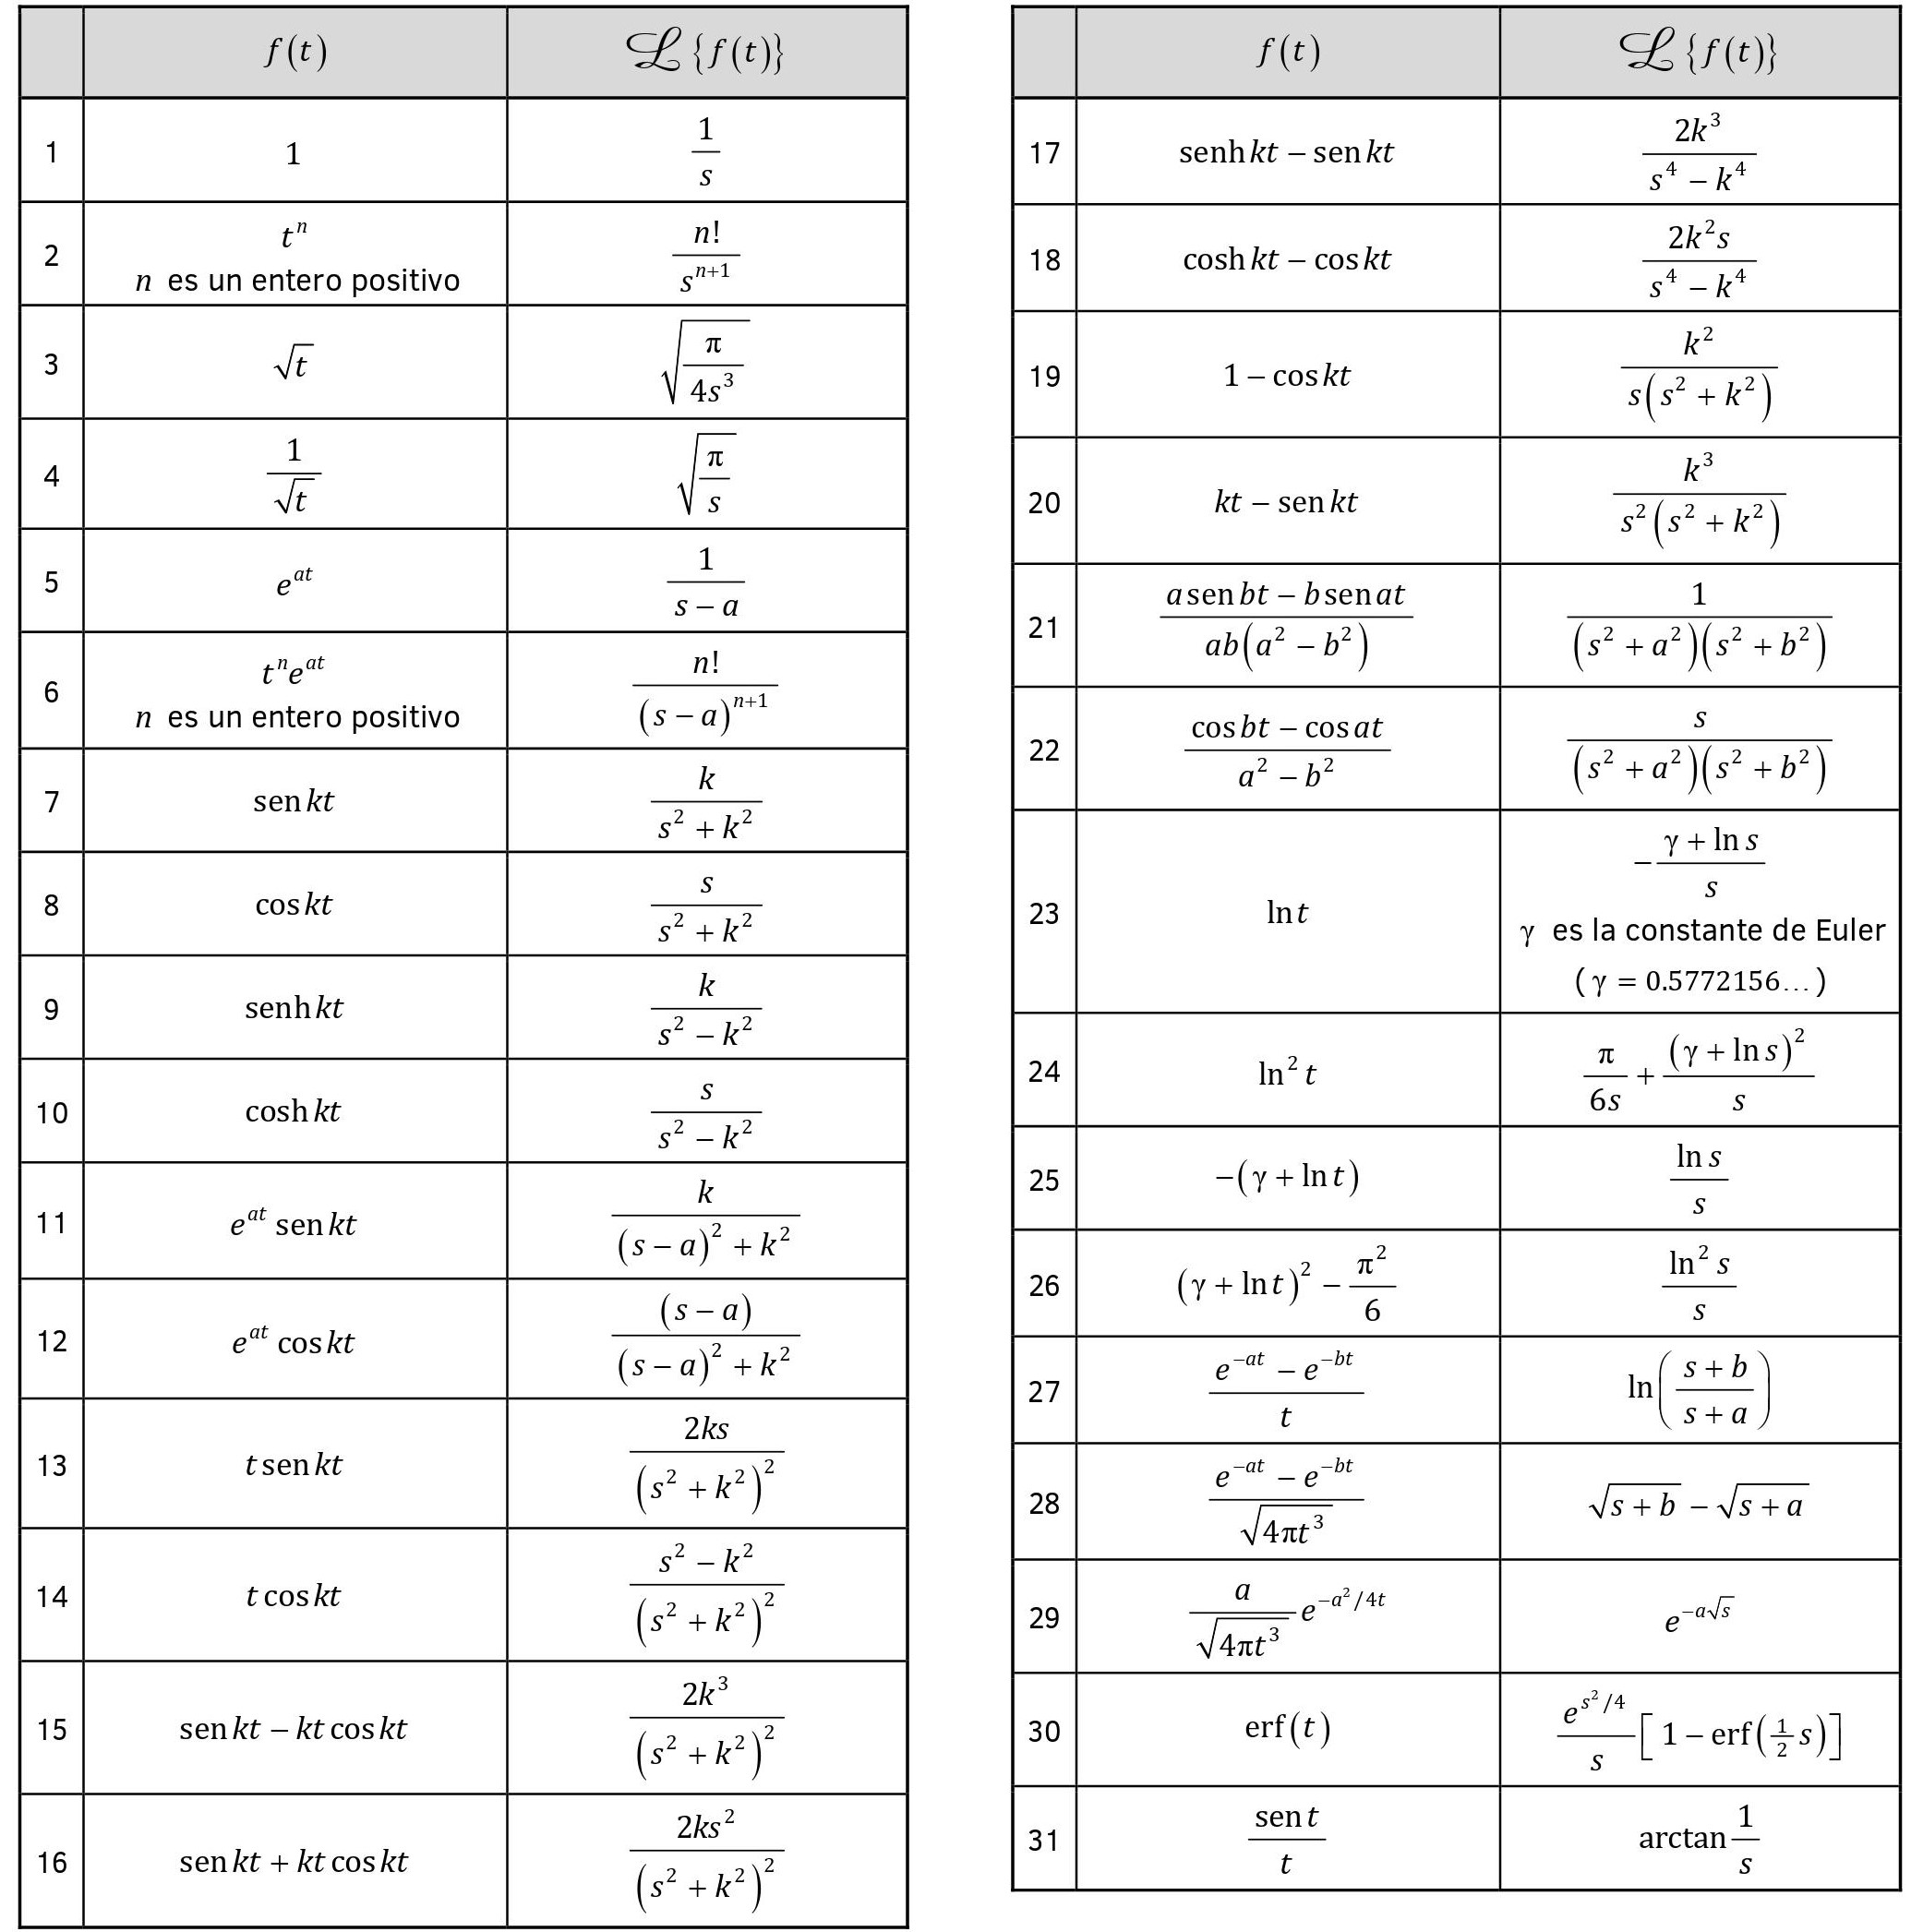
\includegraphics[width=\linewidth]{I2/1.jpg}
\caption{Tabla de transformada de Laplace}
\label{fig:tabla de transformadas Laplace}
\end{figure}
\subsection{Propiedades de la transformada de Laplace}
\begin{theorem}[Producto constante]
Sea \textit{a} un valor constante que multiplica a una función, la transformada de Laplace de esta función será el valor de la constante multiplicada por la transformada de Fourier de esta función:
\begin{equation}
L\llaves{a\cdot f(t)}=a\cdot L\llaves{f(t)}
\end{equation}
\end{theorem}
\begin{example}[Producto constante]
\begin{align*}
&L\llaves{\underbrace{7}_{cte}\cdot\underbrace{\sin(8t)}_{f(t)}}\\
&7\cdot L\llaves{\sin(8t)}\\
&7\cdot\frac{8}{s^2+64}\\
&\frac{56}{s^2+64}
\end{align*}
\end{example}
\begin{theorem}[Linealidad]
La transformada de la adición o sustracción de dos funciones es la suma o sustracción de sus transformadas independientes. De igual manera se aplica la propiedad anterior:
\begin{equation}
L\llaves{a\cdot f(t)\pm b\cdot g(t)}=a\cdot L\llaves{f(t)}\pm b\cdot L\llaves{g(t)}
\end{equation}
\end{theorem}
\begin{example}[Linealidad]
\begin{align*}
L\llaves{3t^2-9t}&=L\llaves{3t^2}-L\llaves{9t}
&=3\cdot\frac{2!}{s^3}-9\cdot\frac{1!}{s^2}
&=\frac{6}{s^3}-\frac{9}{s^2}
\end{align*}
\end{example}
\begin{theorem}[Traslación]
Si una función es multiplicada por una exponencial, con un múltiplo real del tiempo, esto provocará una traslación en el plano complejo, de otra manera:
\begin{equation}
L\llaves{e^{a\cdot t}f(t)}=F(s-a), a\in \mathcal{R}
\end{equation}
\end{theorem}
\begin{example}[Traslación]
\begin{align*}
&L\llaves{\underbrace{e^{2t}}_{e^{at},a=2}\cdot\underbrace{\sin(3t)}_{f(t)}}\\
&L\llaves{\sin(3t)}=\frac{3}{s^2+9}=F(s)
&L\llaves{e^{2t}\sin(3t)}=F(s-2)=\frac{3}{(s-2)^2+9}
\end{align*}
\end{example}
\begin{theorem}[Derivada]
Sea una función del tiempo, multiplicada por el tiempo elevado a la enésima potencia; su transformada menos uno elevado a la enésima potencia por la enésima derivada de la transformada de Laplace de la función:
\begin{equation}
\mathscr{L}\llaves{t^n\cdot f(t)}=(-1)^nF^{n'}(s)
\end{equation}
\end{theorem}
\begin{example}[Derivada]
\begin{align*}
\mathscr{L}\llaves{t\cos(7t)}&=?\\
\mathscr{L}\llaves{\cos(7t)}&=\frac{s}{s^2+7^2}=F(s)\\
\mathscr{L}\llaves{t\cos(7t)}&=\textcolor{red}{(-1)^1}F'(s)\\
&=\parentesis{\frac{s}{s^2+49}}'=\frac{1(s^2+49)-s\cdot 2s}{(s^2+49)^2}\\
&=\frac{s^2+49-2s^2}{(s^2+49)^2}=\frac{-s^2+49}{(s^2+49)^2}\\
&\mathscr{L}\llaves{t\cos(7t)}=\textcolor{red}{-}\parentesis{\frac{-s^2+49}{(s^2+49)^2}}
\end{align*}
\end{example}
\subsection{Transformada de la función escalón unitario o Heaviside}
\begin{wrapfigure}{l}{0.5\linewidth}
  \begin{center}
    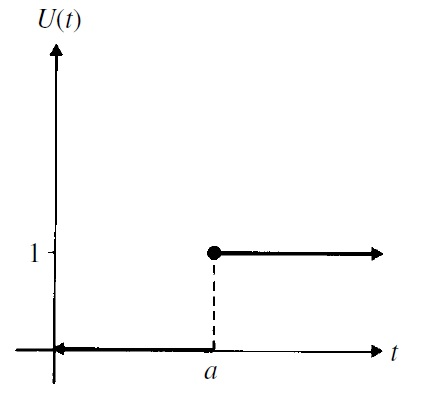
\includegraphics[width=.95\linewidth]{I2/2.jpg}
  \end{center}
  \caption{Función escalón unitario}
\end{wrapfigure}
Definida analíticamente como:
\begin{equation*}
f(t) = \left\lbrace
\begin{array}{ll}
\textup{si } t>a & 1\\
\textup{si } t\leq a & 0
\end{array}=u(t-a)=H(t-a)
\right.
\end{equation*}
Su transformada de Laplace de un escalón unitario es:
\begin{displaymath}
\mathscr{L}\llaves{u(t-a)}=\frac{e^{-a\cdot s}}{s}
\end{displaymath}
Calculando la transformada de Laplace de H(t-3):
\begin{displaymath}
\mathscr{L}\llaves{H(t-3)}=\frac{e^{-3\cdot s}}{s}
\end{displaymath}
Hasta esta parte resulta fácil, sin embargo se suele mezclar más funciones escalón unitario para crear un pulso rectangular, haremos ambos casos:
\subsubsection{Pulso rectangular}
\begin{wrapfigure}{l}{0.5\linewidth}
  \begin{center}
    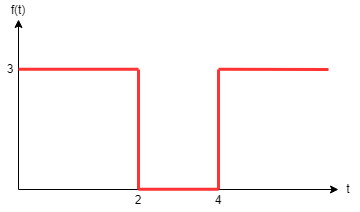
\includegraphics[width=.95\linewidth]{I2/3.png}
  \end{center}
  \caption{Función pulso rectangular: caso 1}
\end{wrapfigure}
Para entender el como se caracteriza esta función usando pulsos unitarios, vamos a empezar analizando desde 0 hasta el infinito. Tenemos un punto de cambio en 3, para números menores a 3 la función vale cero, mientras que para pulsos mayores a 3 debería valer 1; sin embargo en la gráfica se muestra valor constante en 7. Esto se soluciona multiplicando la función escalón unitario por 7; si lo hacemos, para números menores antes de 3 tendremos o ($7\times 0$) y para mayores a 3 tendremos 7 ($7\times 1$). Por lo tanto tenemos:
\begin{displaymath}
7\cdot u(t-3)
\end{displaymath}
El comportamiento visto sería al infinito positivo, pero notamos que en 5 se hace cero. Lo analizamos de la siguiente manera, para antes del 5 es 7, que ya fue caracterizado, por lo tanto no debemos alterar nada; mientras que para números mayores a 5 vale 0, cosa que cambia pues fue caracterizada como 7. Bajo estas ideas podemos restar una función escalón unitario a la función ya hecha, ojo que esta función a restar deber ser escalada por 7, si no la escalamos tendríamos solo 7-1=6, cuando debería ser 7-7=0:
\begin{displaymath}
f(t)=7\cdot u(t-3)-7\cdot u(t-5)
\end{displaymath}
De esta manera se ha caracterizado la función pulso rectangular usando funciones heaviside, ahora se puede calcular su transformada de Laplace:
\begin{align*}
\mathscr{L}\llaves{7\cdot u(t-3)-7\cdot u(t-5)}&=\mathscr{L}\llaves{7\cdot u(t-5)}-\mathscr{L}\llaves{7\cdot u(t-5)}\\
&=7\cdot\mathscr{L}\llaves{u(t-5)}-7\cdot\mathscr{L}\llaves{u(t-5)}\\
&=7\cdot\frac{e^{-3s}}{s}-7\cdot\frac{e^{-5s}}{s}
\end{align*}

Para el caso 2, sabiendo como es la función escalón unitario, nos dice que para antes de 2 debe valer 3 y para valores después de 2 debe ser 0. Para caracterizarlo, empezamos con una función constante \textcolor{red}{3}:
\begin{align*}
&t\leq 2\rightarrow \textcolor{red}{3}-0=3\\
&t>2\rightarrow \textcolor{red}{3}-1=2
\end{align*}
Nota que a la función constante 3 le estamos restando una función escalón unitario, sin embargo despues de 2 NO nos da 0, nos da 2. Esto se arregla escalando la función \textcolor{blue}{Heaviside}:
\begin{align*}
&t\leq 2\rightarrow \textcolor{red}{3}-\textcolor{blue}{3}\cdot 0=3\\
&t>2\rightarrow \textcolor{red}{3}-\textcolor{blue}{3}\cdot 1=0
\end{align*}
Analíticamente:
\begin{displaymath}
f(t)=3-3\cdot u(t-2)
\end{displaymath}
\begin{wrapfigure}{r}{0.4\linewidth}
  \begin{center}
    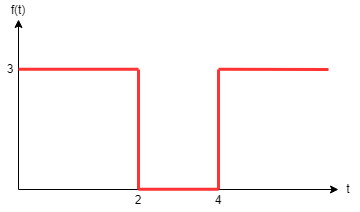
\includegraphics[width=.95\linewidth]{I2/3.png}
  \end{center}
  \caption{Función pulso rectangular: caso 2}
\end{wrapfigure}
Ahora para el punto 4, solo debemos sumar una función heaviside simple, escalada en 3 y desplazada hasta t=4, por lo tanto:
\begin{displaymath}
f(t)=3-3\cdot u(t-2)+3\cdot u(t-4)
\end{displaymath}
Ahora se resuelve la transformada de esta función:
\begin{align*}
&\mathscr{L}\llaves{f(t)=3-3\cdot u(t-2)+3\cdot u(t-4)}\\
&\mathscr{L}\llaves{3}-3\mathscr{L}\llaves{u(t-2)}+3\mathscr{L}\llaves{u(t-4)}\\
&=\frac{3}{s}-3\frac{e^{-2s}}{s}+3\frac{e^{-4s}}{s}
\end{align*}




\section{Transformada de Fourier}

\section{Transformada Z}
%------------------------------------------------------------
\end{document}
%----------------------------------------------------------------------------------------
